%!TEX root = main.tex

% =============================================================================
\section{Model Evaluation}
\label{sec:model-evaluation}
% =============================================================================

Using the uncertainty benchmark defined in Section~\ref{sec:uncertainty-benchmark},
    and the analytical cost model from Section~\ref{sec:tuning_lsm_trees},
    we now rigorously evaluate the performance of the proposed robust tunings by
    {\Endure}.

\subsection{Evaluation Metrics}
Now, we describe the metrics used to compare different tuning configurations.

\Paragraph{Normalized Delta Throughput ($\Delta$)} Defining throughput as the 
    reciprocal of the cost of executing a workload, we measure the
    normalized delta throughput of a configuration {$\configuration_2$}
    wrt. another configuration {$\configuration_1$} for a given 
    workload {\workload} as follows, 
    \[
        \Delta_{\workload}(\configuration_1, \configuration_2) = 
        \frac{\nicefrac{1}{C(\workload, \configuration_2)} -
            \nicefrac{1}{C(\workload, \configuration_1)}}
            {\nicefrac{1}{C(\workload, \configuration_1)}}.
    \]
$\Delta_{\workload}(\configuration_1, \configuration_2) > 0$ implies that
    {$\configuration_2$} outperforms {$\configuration_1$} when executing
    a workload {\workload} and vice versa when
    $\Delta_{\workload}(\configuration_1, \configuration_2) < 0$.

\Paragraph{Throughput Range ($\Theta$)} While normalized delta throughput 
    compares two different tunings, we use the throughput
    range to evaluate an individual tuning ${\configuration}$ 
    wrt. the  benchmark set {\benchmark} as follows,
    \[
        \Theta_{\mathcal{B}}(\configuration) = 
        \max_{\workload_0, \workload_1 \in \mathcal{B}}
            \bigg(\frac{1}{C(\workload_0, \configuration)} 
            - \frac{1}{C(\workload_1, \configuration)}\bigg).
    \]
$\Theta_{\benchmark}(\configuration)$ intuitively captures the best
    and the worst-case outcomes of the tuning {\configuration}.
A smaller value of this metric implies higher consistency in performance.

\begin{figure}
    \centering
    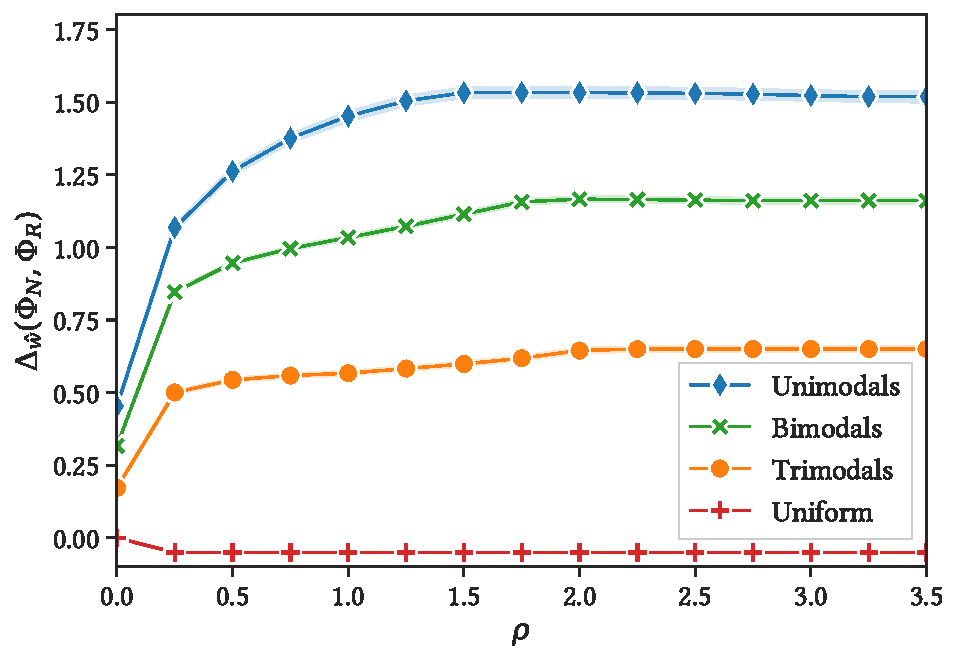
\includegraphics[scale=0.5]{figures/delta_throughput_workload_type.pdf}
    \caption{Delta throughput $\Delta_{\obsworkload}(\Phi_{N}, \Phi_{R})$
        between the nominal and expected tunings across various expected workloads.
    }
    \label{fig:delta_throughput_workload_type}
\end{figure}


\begin{figure*}[ht]
    \centering
    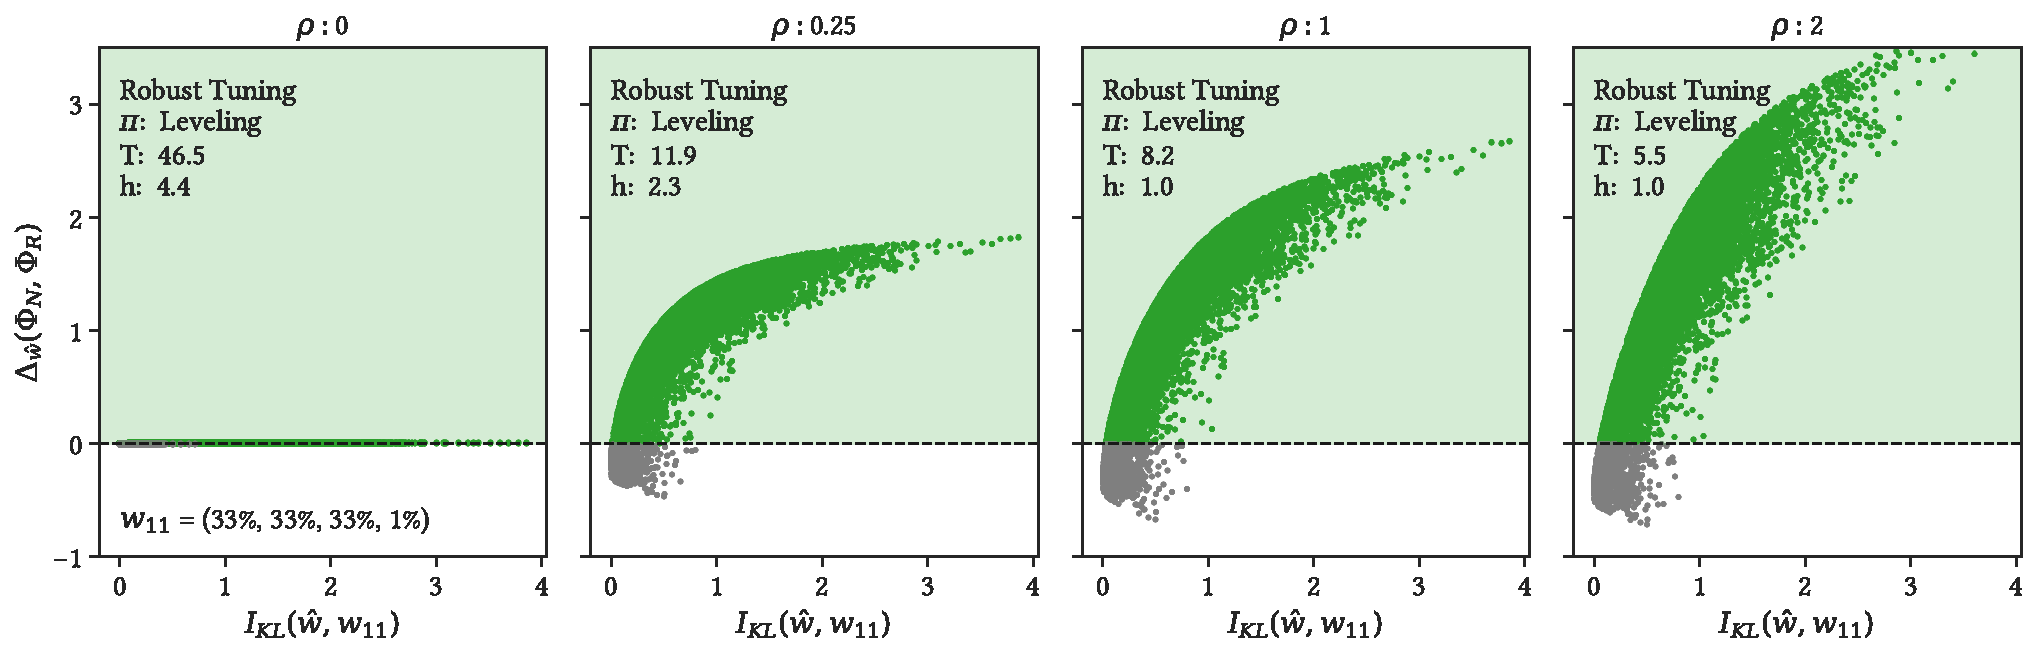
\includegraphics[width=\textwidth]{figures/scatterplot_evolution_rho.pdf}
    \caption{Impact of $\rho$ on normalized delta throughput 
        $\Delta_{\obsworkload}(\Phi_{N}, \Phi_{R})$ for tunings with expected
        workload $\workload_{11}$.
    }
    \label{fig:scatterplot_evolution_rho}
\end{figure*}


\subsection{Experiment Design}

To evaluate the performance of our proposed robust tuning approach, 
    we design a large-scale experiment comparing different tunings
    over the sampled workloads in {\benchmark} using the analytical cost
    model.
For each of the expected workloads in Table \ref{tab:expected-workloads},
    we obtain a single nominal tuning configuration (${\configuration_N}$) by 
    solving the {\nominal} problem. 
For 15 different values of $\rho$ in the range (0.0, 4.0) with a step size of
    0.25, we obtain a set of robust tuning configurations ($\configuration_R$)
    by solving the {\robustw} problem.
Finally, we individually compare each of the robust tunings with the nominal
    over the 10,000 workloads in {\benchmark} to obtain over 2 million
    comparisons.
While computing the costs, we assume that the database contains 10 million
    entries each of size 1 KB. 
Analysis presented in the following sections assumes a total available memory of
    10 GB.
In the following sections, for brevity purposes, we present representative 
    results  corresponding to individual expected workloads and specific system 
    parameters.
However, we exhaustively confirmed that changing these parameters do not 
    qualitatively affect the outcomes of our experiment.

\subsection{Results}
\label{sec:model-results}
Here, we present an analysis of the comparisons between the robust and 
    the nominal tuning configurations.
Using an off-the-shelf global minimizer from the popular Python optimization
    library SciPy \cite{2020SciPy-NMeth}, we obtain both nominal and robust
    tunings with the runtime for the above experiment being less than 10
    minutes.
% Our code has been made publicly available in order to encourage reproducible
%     research \cite{??}.

\Paragraph{Comparison of Tunings}
First, we address the question -- \textit{is it beneficial to adopt robust tunings
    relative to the nominal tunings?}
Intuitively, it should be clear that the performance of nominally tuned databases
    would degrade when the workloads being executed on the database are 
    significantly different from the expected workloads used for tuning.
In Figure~\ref{fig:delta_throughput_workload_type},
    we present performance comparisons between the robust and the nominal 
    tunings for different values of uncertainty parameter $\rho$.
We observe that robust tunings provide substantial benefit in terms of normalized
    delta throughput for \emph{unimodal}, \emph{bimodal}, and \emph{trimodal} 
    workloads.
The normalized delta throughput 
    $\Delta_\obsworkload(\configuration_N, \configuration_R)$
    shows over 95\% improvement on average over all $\obsworkload \in \benchmark$ 
    for robust tunings with $\rho \geq 0.5$, 
    when the expected workload used during tuning belongs to one of these 
    categories.
For \emph{uniform} expected workload, we observe that the nominal tuning outperforms the 
    robust tuning by a modest 5\%.

Intuitively, \emph{unbalanced} workloads result in overfit nominal tunings.
Hence, even small variations in the observed workload can lead to 
    significant degradation in the throughput of such nominally tuned databases. 
On the other hand, robust tunings by their very nature take into account such
    variations and comprehensively outperform the nominal tunings.
In case of the uniform expected workload $\workload_0$, 
    Figure ~\ref{fig:KL_divergence_histogram} shows us that instances of 
    high values of KL-divergence are extremely rare.
In this case, when tuned for high values of $\rho$, the robust tunings are 
    unrealistically pessimistic and lose out some performance relative to the 
    nominal tuning.

\Paragraph{Impact of Tuning Parameter $\rho$}
Next, we address the question -- \emph{how does the uncertainty tuning parameter
    $\rho$ impact the performance of the robust tunings?}
In Figure~\ref{fig:scatterplot_evolution_rho}, we take a deep dive into
    the performance of robust tunings for an individual
    expected workload for different values of $\rho$.
We observe that the robust tunings for $\rho=0$ i.e., zero uncertainty, are 
    very close to the nominal tunings.
As the value of $\rho$ increases,
    its performance advantage over the nominal tuning for the observed 
    workloads with higher KL-divergence wrt. expected workload
    increases.
Furthermore, the robustness of such configurations have logically sound 
    explanations.
The expected workload in 
    Figure~\ref{fig:scatterplot_evolution_rho} consists of just 1\% writes.
Hence, for low values of $\rho$, the robust tuning has higher size-ratio leading to
    shallower LSM trees to achieve good read performance.
For higher values of $\rho$, the robust tunings anticipate increasing
    percentage of write queries and hence limit the size-ratio to achieve overall
    higher throughput.

\begin{figure*}[htbp]
    \centering
    \begin{subfigure}[h]{0.74\textwidth}
        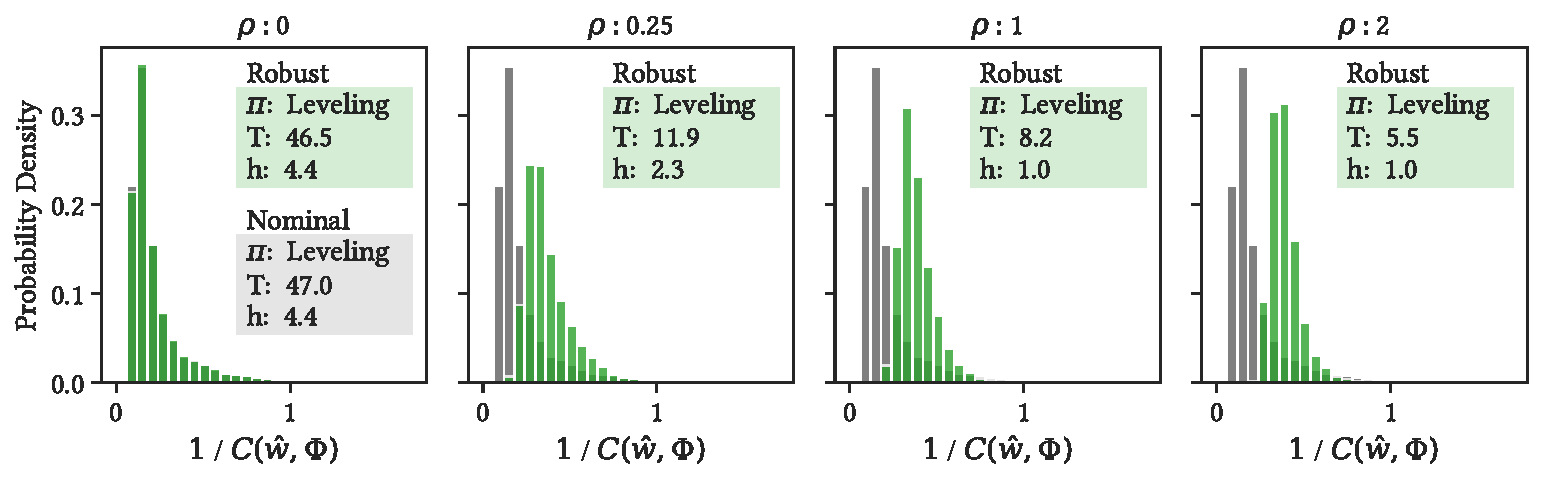
\includegraphics[scale=0.5]{figures/overlapping_histogram.pdf}
        \caption{Histograms of throughput $1 / C(\obsworkload, \Phi)$ for
            tunings with expected workload $\workload_{11}$ }
        \label{fig:overlapping_histogram}
    \end{subfigure}
    \begin{subfigure}[h]{0.24\textwidth} 
        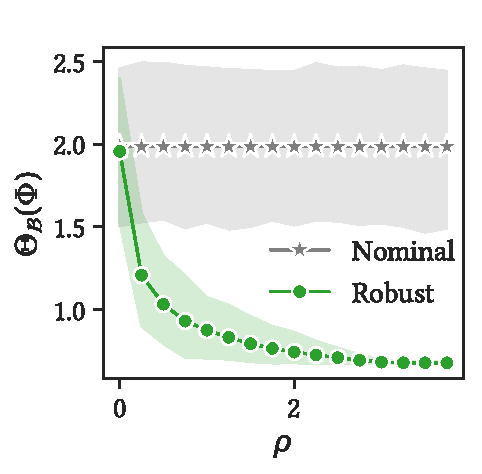
\includegraphics[scale=0.5]{figures/throughput_range_evolution.pdf}
        \caption{Throughput range $\Theta_{\mathcal{B}}(\Phi)$}
        \label{fig:throughput_range_evolution}
    \end{subfigure}
    \caption{Impact of $\rho$ on throughput.}
    \label{fig:rho_throughput_range_impact}
\end{figure*}

In Figure~\ref{fig:rho_throughput_range_impact}, we show the impact of tuning
    parameter $\rho$ on the throughput range.
Specifically, in Figure~\ref{fig:overlapping_histogram} we plot a histogram of 
    the nominal and robust throughputs for workload $\workload_{11}$. 
As the value of $\rho$ increases, the interval size between the lowest and the 
    highest throughputs for the robust tunings consistently decreases.
We provide further evidence of this phenomenon in 
    Figure~\ref{fig:throughput_range_evolution}, by plotting the decreasing  
    throughput range $\Theta_\benchmark(\configuration_R)$  
    averaged across all the expected workloads. 
Thus, robust tunings not only provide a higher average throughout over all 
    $\obsworkload \in \benchmark$, 
    but also a more consistent performance with lower variance when compared
    to the nominal tunings.

\Paragraph{Choice of Tuning Parameter $\rho$} Now, we address the question -- 
\emph{What is the appropriate choice for the value of uncertainty parameter $\rho$?}
We provide guidance on the choice of $\rho$ in absence of perfect knowledge
    regarding the future workloads that are likely to be executed on the
    database.
Intuitively, we expect the robust tunings to be only weak when they are tuned 
    for either too little or too much uncertainty.
In Figure~\ref{fig:rho_vs_rho_hat}, we explore the relationship between $\rho$
and the KL-divergence $I_{KL}(\obsworkload, \workload)$ for 
    $\obsworkload \in \benchmark$, 
    by making a contour plot of the corresponding normalized delta throughput
    $\Delta_{\obsworkload}(\configuration_N, \configuration_R)$.
We confirm our intuition that nominal tunings compare favorably with our
    proposed robust tunings only in two scenarios viz., (1) when observed workloads
    are extremely similar to the expected workload (close to zero observed 
    uncertainty),
    and (2) when the robust tunings assume extremely low uncertainty with 
    $\rho < 0.2$ while the observed variation in workloads is higher.
Based on this evidence, we can advise a potential database administrator that
    mean KL-divergences between pairs of historically observed workloads would
    be a reasonable value of $\rho$ while deploying robust tunings in practice.

\begin{figure}[h]
    \centering
    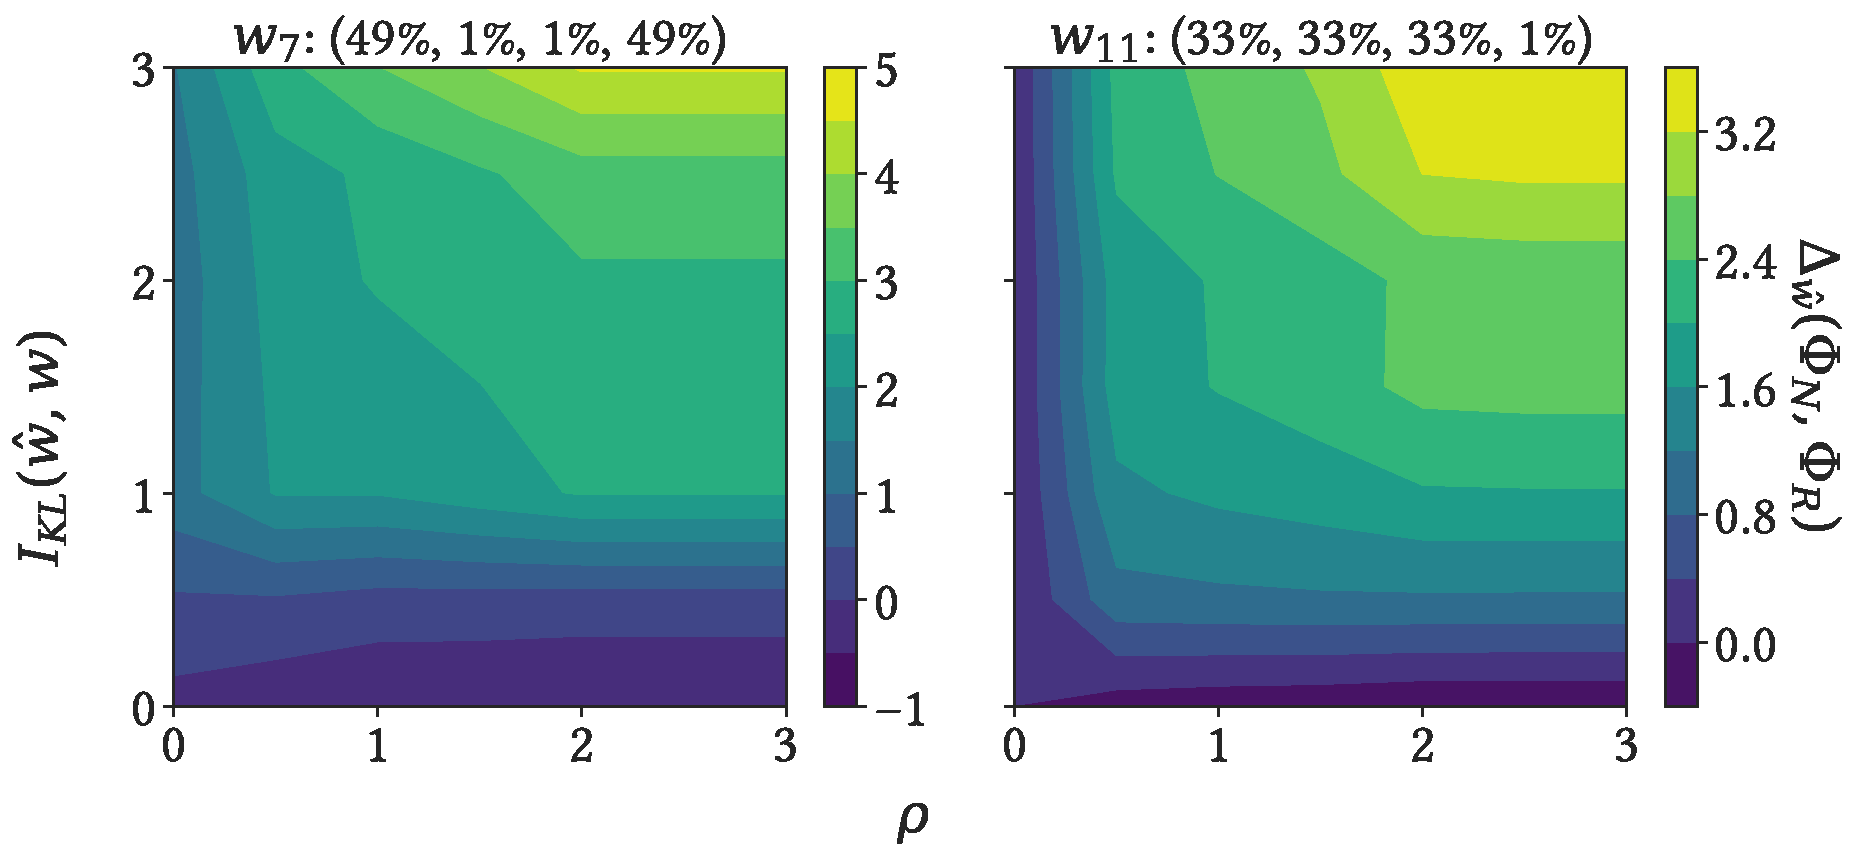
\includegraphics[scale=0.25]{figures/rho_vs_rho_hat.pdf}
    \caption{Delta throughputs $\Delta_{\obsworkload}(\Phi_{N},
        \Phi_{R})$ for $\rho$ vs $I_{KL}(\obsworkload, \workload)$.}
    \label{fig:rho_vs_rho_hat}
\end{figure}
